\chapter{Operatori compatti e autoauggiunti}

\section{Operatore aggiunto e operatori aggiunti}
Sia $(E, (\cdot, \cdot))$ uno spazio con prodotto scalare.
Fissato $y \in H$, consideriamo la funzione $R_y : H \to \C$ definito come
\begin{equation*}
	R_y x = (x,y).
\end{equation*}
Sappiamo che tale operatore è lineare e continuo, di norma unitaria, e dunque è un'isometria. Dunque la funzione $y \mapsto R_y$ da $E$ a $E'$ è un'isometria \emph{anti}lineare (perchè il secondo argomento del prodotto scalare è antilineare).

\begin{theorem}
\label{eq:ops_riesz}
	Sia $(H, (\cdot,\cdot))$ di Hilbert.
	Allora la mappa $R_-: H \to H'$ definita come $y \mapsto (-, y)$ è un'isometria suriettiva.
\end{theorem}
\begin{proof}
	Sappiamo già che la funzione $R_-$ è un'isometria. Rimane da dimostrare la suriettività.
	Senza perdita di generalità, prendiamo $T \in H'$ non nullo (in tal caso, infatti, banalmente $T=R_0$).
	In questo caso, $\ker T \lneq H$, quindi $\dim \im T \geq 1$ e pertanto $T$ è suriettivo poichè $\dim \C = 1$.
	Per il primo teorema di isomorfismo, $H/\ker T \iso \C$, ossia $\dim(\ker T)^\perp = 1$.
	Prendiamo allora $z \in (\ker T)^\perp$, di norma unitaria.
	Sia $x \in (\ker T)^\perp$, abbiamo $Tx = \alpha Tz$ per un certo $\alpha \in \C$, da cui $T(x-\alpha z) = 0$, ossia $x-\alpha z \perp z$, che significa
	\begin{equation*}
		(x-\alpha z, z) = (x,z) - \alpha \cancelto{1}{(z,z)} = 0,
	\end{equation*}
	cioè $(x,z) = \alpha$. Segue che $Tx = \alpha Tz = (x,z)Tz = (x, \conj{Tz}\, z)$, e quindi $T = R_{\conj{Tz} z}$ (infatti anche se $x \in \ker T$, $R_{\conj{Tz} }(x) = 0$).
\end{proof}

\begin{remark}
	Il teorema utilizza la completezza di $H$ quando si assume che ${H = \ker T \oplus (\ker T)^\perp}$. Questo è vero solo se $H$ è di Hilbert: il Teorema~\ref{th:hilb_ort_decomp} si rifà al Teorema~\ref{th:hilb_projector_subspace}, che a sua volta segue dal Lemma~\ref{lemma:hilb_proj}, che è dimostrato dal teorema della proiezione (Teorema~\ref{th:hilb_projection}) il quale usa in maniera essenziale la completezza.
\end{remark}

\begin{corollary}
	Sia $\{x_n\}_{n \in \N}$ una successione in uno spazio di Hilbert $H$.
	Allora $x_n \weakconv x$ se e solo se $(x_n, y) \conv (x,y)$ per ogni $y \in H$.
\end{corollary}

\begin{corollary}
	Sia $\{u_n\}_{n \in \N}$ una successione ortonormale in uno spazio di Hilbert $H$.
	Allora $u_n \weakconv 0$, anche se $u_n \not\conv 0$.
\end{corollary}
\begin{proof}
	Per Bessel,
	\begin{equation*}
		\lim_n (x, u_n) = 0, \qquad \text{per ogni $x \in H$}.
	\end{equation*}
	Dunque la tesi segue dal precedente. Infine la convergenza forte non sussiste in quanto $\|u_n\| = 1$ per ogni $n \in \N$.
\end{proof}

\begin{definition}
	Sia $H$ uno spazio di Hilbert, e sia $T:H \to H$ lineare e continuo.
	Un operatore $T^* : H \to H$ si dice \defining{aggiunto} di $T$ se
	\begin{equation*}
		(Tx, y) = (x T^* y), \qquad \text{per ogni $x,y \in H$}.
	\end{equation*}
\end{definition}

\begin{definition}
	Si dice \defining{autoauggiunto} un operatore che coincide col proprio aggiunto.
\end{definition}

\begin{lemma}
	Ogni operatore $T:H \to H$ ammette aggiunto, lineare e continuo e si ha $\|T^*\|=\|T\|$.
\end{lemma}
\begin{proof}
	Sia $f_y : H \to \C$ definita come $x \mapsto (Tx, y)$. Essa è banalmente lineare e continua. Dal teorema di rappresentazione di Riesz, esiste $y^* \in H$ tale che $f_y(x) = (Tx,y) =(x, y^*)$. Dunque poniamo $T^* y = y^*$. La linearità di questo operatore è evidente, ed inoltre è limitato:
	\begin{equation*}
		\|T^* y\| = \|y^*\| = \|f_y\| \leq \|T\|\|y\|.
	\end{equation*}
	In particolare abbiamo dimostrato che $\|T^*\| \leq \|T\|$. Per vedere l'altra disuguaglianza, si noti che $(T^{**} = T$, infatti
	\begin{equation*}
		(T^*x, y) = \conj{(y, T^*x)} = \conj{(Ty, x)} = (x, Ty)
	\end{equation*}
	Dunque $\|T^*\| \leq \|T^{**}\| = \|T\|$.
\end{proof}

\begin{exercise}
	Se $T,S:H \to H$ e $\alpha \in \C$, allora:
	\begin{enumerate}
		\item $1^* = 1$,
		\item $0^* = 0^*$,
		\item $(S+T)^* = S^* + T^*$,
		\item $(\alpha T)^* = \conj\alpha T^*$,
		\item $(ST)^* = T^*S^*$.
	\end{enumerate}
\end{exercise}

\begin{example}
	Nel caso finito, se rappresentiamo un operatore $T: \C^n \to \C^n$ con una matrice $A$, allora $T^*$ è rappresentato da $A^\dagger$, ossia $\conj{A^T}$:
	\begin{equation*}
		(Tx,y) = \conj{y}^T A x = x^T A^T \conj{y} = (x, \conj{A^T y}), \qquad \text{per ogni $x,y \in \C^n$}.
	\end{equation*}
\end{example}

\begin{example}[Operatori integrali di Fredholm e Volterra]
	Sia $H = L^2(a,b)$, con $a < b$, e sia $K \in L^2((a,b) \times (a,b))$. Si definisce
	\begin{eqalign*}
		T :L^2(a,b) &\longto L^2(a,b)\\
			f &\longmapsto \int_a^b K(s,t)\,f(t)\,\dt.
	\end{eqalign*}
	Si ha
	\begin{eqalign*}
		T^* :L^2(a,b) &\longto L^2(a,b)\\
			f &\longmapsto \int_a^b \conj{K(t,s)}\,f(t)\,\dt.
	\end{eqalign*}
	Essi sono ben definiti, in quanto:
	\begin{eqalign*}
		|Tf(t)| \leq \int_a^b |K(s,t)|\,|f(t)|\,\dt
		\underset{\text{C-S}}= \left(\int_a^b |K(s,t)|^2\,\dt \right)^{1/2}\!\left( \int_a^b |f(t)|^2\,\dt \right)^{1/2}\\[1ex]
		\left(\int_a^b |Tf(t)|^2\,\dt \right)^{1/2} \leq \left( \int_a^b\int_a^b |K(t,s)|^2\,\ds\,\dt\right)^{1/2}\,\left( \int_a^b |f(t)|^2\,\dt \right)^{1/2}
	\end{eqalign*}
	Per cui:
	\begin{equation*}
		\|Tf\|_{L^2} \leq \|K\|_{L^2} \|f\|_{L^2}.
	\end{equation*}
	Verifichiamo ora che $T^*$ sia l'aggiunto di $T$:
	\begin{eqalign*}
		(Tf,g)_{L^2} &= \int_a^b \int_a^b K(t,s)\,f(s)\,\ds\, \conj{g(t)}\,\dt\\
		&\underset{Fub.}= \int_a^b \int_a^b K(t,s) \,\conj{g(t)}\,\dt\,f(s)\,\ds\\
		&= \int_a^b f(s)\, \conj{\int_a^b \conj{K(t,s)} \,g(t)\,\dt}\,\ds\\
		&= (f, {\textstyle \int_a^b} \conj{K(t,s)}\,g(t)\,\dt).
	\end{eqalign*}
\end{example}

\begin{remark}
	Il nucleo $K$ si può considerare come `matrice infinita'. Se questa matrice è triangolare inferiore, ossia se $K(t,s) = 0$ per ogni $s>t$, allora $T$ si chiama \defining{operatore di Volterra}.
\end{remark}

\begin{lemma}
	Sia $H$ di Hilbert, sia $T : H \to H$ lineare e continuo.
	Allora
	\begin{equation*}
		\ker T = (\im T^*)^\perp, \qquad (\ker T)^\perp = \closure{\im T^*}.
	\end{equation*}
\end{lemma}
\begin{proof}
	Sia $x \in \ker T$, allora $(x, T^*y) = (Tx, y)=0$, quindi $x \in (\im T^*)^\perp$.
	D'altra parte, se $x \in (\im T^*)^\perp$ allora $0 = (x, T^*y) = (Tx,y)$ per ogni $y \in H$, cioè $Tx = 0$.
	Infine, dalla prima segue che $(\ker T)^\perp = (\im T^*)^{\perp\perp} = \closure{\im T^*}$.
\end{proof}

\begin{remark}
	Nel precedente, $\closure{-}$ indica la chiusura. Questo perchè dal Lemma~\ref{lemma:hilb_ort_comp} segue che se $S \leq H$, allora $S^{\perp\perp} = \closure{S}$.
\end{remark}

\begin{theorem}
	Sia $H$ spazio di Hilbert \emph{complesso}, $T:H \to H$ lineare e continuo.
	Allora $T$ è autoauggiunto se e solo se $(Tx, x) \in \R$ per ogni $x \in H$.
\end{theorem}
\begin{remark}
	Questo fatto deriva da ragioni spettarli (si pensi al caso finito-dimensionale).
\end{remark}
\begin{proof}
	\leavevmode
	\begin{description}
		\item[$(\Longrightarrow)$] Si fissi $x \in H$. Siccome $(Tx,x) = (x,Tx) = \conj{(Tx,x)}$, segue che tale numero debba essere reale.
		\item[$(\implied)$] Per le forme sesquilineari su spazi complessi vale la seguente formula `di polarizzazione':
		\begin{equation*}
			4 (Tx,y) = (T(x+y),x+y) - (T(x-y), x-y) + i\left[ (T(x+iy),x+iy) - (T(x-iy), x-iy) \right].
		\end{equation*}
		Ora, siccome $(Tx,x) \in \R$ per ogni $x \in H$, possiamo scambiare gli argomenti senza dover coniugare. Se facciamo ciò nella formula appena scritta, è evidente che otteniamo $4(x,Ty)$, perciò abbiamo provato che $T$ è autoauggiunto.
	\end{description}
\end{proof}

Un altro approccio per gestire la compattezza negli spazi infinito-dimensionale è usare la seguente nozione di operatore:

\begin{definition}
	Siano $E$, $F$ spazi normati e $T:E \to F$ una funzione.
	Diciamo che $T$ è un \defining{operatore compatto} se è lineare, e per ogni successione $\{x_n\}_{n \in \N}$ limitata in $E$ esiste una sottosuccessione la cui immagine secondo $T$ converge in $F$. Equivalentemente, per ogni $A \subseteq E$ limitato, si ha $T(A)$ è relativamente compatto.
\end{definition}

\begin{example}[\emph{L'identità è il nemico numero uno della compattezza.}]
	Se $\dim E = \infty$, allora $1_E : E \to E$ \underline{non} è compatta! Infatti sappiamo che $\closure{B}_E(0,1)$ non è compatta (Teorema~\ref{th:unit_ball_not_compact}).
\end{example}

\begin{exercise}
	Sia $T:E \to F$ lineare compatto. Allora $T$ è continuo.

	\textbf{Svolgimento}. $T$ manda insiemi limitati in insiemi limitati (compatto $\implies$ limitato anche in dimensione infinita). Quindi $T$ è limitato, ergo continuo.
\end{exercise}

\begin{exercise}
	Provare che la composizione di operatori compatti è compatta.
\end{exercise}

\begin{exercise}
	Sia $T:E \to F$, $\dim E = \infty$, $T$ lineare, continuo e con inversa continua.
	Allora $T$ non è compatto.

	\textbf{Svolgimento}. Dall'esercizio precedente sappiamo che la composizione di compatti è compatta. Ma $TT^{-1} = 1_F$, che non è compatto.
\end{exercise}

\begin{theorem}
	Siano $E$, $F$ spazi normati.
	\begin{enumerate}
		\item Se $T:E \to F$ è compatto, e $x_n \weakconv x$ in $E$, allora $Tx_n \conv Tx$ in $F$, ossia gli operatori compatti mandano successioni debolmente convergenti in successioni fortemente convergenti.
		\item Se $E$ è riflessivo e $T:E \to F$ manda successioni debolmente convergenti in successioni fortemente convergenti, allora $T$ è compatto.
	\end{enumerate}
\end{theorem}
\begin{proof}
	\leavevmode
	\begin{enumerate}
		\item Per dimostrare che $Tx_n \conv Tx$ basta dimostrare che da ogni sottosuccessione di $\{Tx_n\}_{n \in \N}$ si può estrarre un'altra sottosuccessione convergente a $Tx$.
		Sia $\{x_{n_h}\}_{h \in \N}$ una sottosuccessione di $\{x_n\}_{n \in \N}$. Per compattezza, esiste una sottosuccessione di $\{Tx_{n_h}\}_{h \in \N}$ che converge a $y \in F$. Rimane da mostrare che $y =Tx$. Si osservi che per $\varphi \in F'$, $\varphi(Tx_{n_{h_k}}) \conv \varphi(y)$, cioè $\varphi T \in E'$ preserva la convergenza. Ma siccome $\{x_n\}_{n \in \N}$ converge debolmente, $\varphi T(x_{n_{h_k}}) \conv \varphi T(x)$. Segue che $\varphi T(x) = \varphi(y)$ per ogni $\varphi \in F'$, quindi $Tx=y$.

		\item Sia $\{x_n\}_{n \in \N}$ successione limitata in $E$. Essendo $E$ riflessivo, esiste una sua estratta che converge debolmente, per cui $Tx_{n_h} \conv Tx$ per il punto precedente.
	\end{enumerate}
\end{proof}

\begin{example}[Operatore di Fredholm]
	Siano $a <b \in \R$, $K \in \Czero([a,b] \times [a,b])$. Definiamo l'operatore $T:L^2(a,b) \to L^2(a,b)$:
	\begin{equation*}
		Tf(t) = \int_a^b K(t,s)\,f(s)\,ds.
	\end{equation*}
	Allora $T$ è compatto.

	\textbf{Svolgimento}.
	Infatti $Tf \in \Czero[a,b]$. Sia $\{f_n\}_{n \in \N}$ in $L^2(a,b)$, limitata. Proviamo che $\{Tf_n\}_{n \in \N}$ è equilimitata ed equicontinua in $[a,b]$.
	\begin{enumerate}
		\item Equilimitatezza:
		\begin{eqalign*}
			|Tf_n(t)| &= \left| \int_a^b K(t,s)\,f_n(s)\,ds \right|\\
			&\leq \max_{[a,b] \times [a,b]} K\ \int_a^b |f_n(s)|\,ds\\
			&\underset{\text{H\"o}}\leq \max_{[a,b] \times [a,b]} K\ (b-a)^{1/2}\ \left( \int_a^b |f_n(s)|^2 \,ds \right)^{1/2}\\
			&\leq M, \qquad \text{per ogni $n \in \N$}.
		\end{eqalign*}
		\item Equicontinuità. Siccome $K$ è continua su un compatto, lo è uniformemente. Dunque fissato $\varepsilon > 0$, esiste $\delta > 0$ tale che
		\begin{equation*}
			|t_1-t_2| < \delta,\ |s_1, s_2| < \delta \implies |K(t_1,s_1) - K(t_2, s_2)| \leq \varepsilon.
		\end{equation*}
		Si ha
		\begin{eqalign*}
			|Tf_n(t_1) - Tf_n(t_2)| &\leq \int_a^b |K(t_1,s) - K(t_2, s)|\,|f_n(s)|\,\ds\\
			&\leq \varepsilon \int_a^b \,|f_n(s)|\,\ds\\
			&\leq \varepsilon \,|b-a|^{1/2} \, \|f_n\|_{L^2}\\
			&\leq \varepsilon M, \qquad \text{per ogni $n \in \N$}.
		\end{eqalign*}
	\end{enumerate}
	Dal teorema di Ascoli--Arzelà dunque, esiste una sottosuccessione $Tf_{n_m}$ che converge uniformemente a $g \in Czero[a,b]$, e pertanto converge in $L^2(a,b)$ ad una funzione $L^2(a,b)$.
\end{example}

\begin{theorem}
	Siano $E$, $F$ spazi normati, $F$ di Banach. Lo spazio $K(E,F)$ degli operatori compatti $E \to F$ è chiuso in $E \to F$.
\end{theorem}
\begin{remark}
	Questo ci permette poi di dire che una successione convergente di operatori compatti ha limite compatto.
\end{remark}
\begin{proof}
	Sia $\{T_n\}_{n \in \N}$ una successione di operatori compatti, tali che $T_n \conv T \in E \to F$ in norma operatoriale.
	Sia ora $\{x_n\}_{n \in \N}$ una successione limitata in $E$. Diagonalizziamo $\{T_mx_n\}_{m, n \in \N}$ raffinando gli indici delle estratte convergenti progredendo con $m \in \N$.
	La diagonale così ottenuta, che chiamiamo $\{y_n\}_{n \in \N}$, ha la proprietà che $T_m(y_n)$ converge rispetto ad $n$.
	Proviamo oa che $\{Ty_n\}_{n \in \N}$ mostrando che è di Cauchy.
	Si fissi $\varepsilon > 0$, allora esiste $\bar n \in \N$ tale che $\|T-T_{\bar n}\| z < \varepsilon$. Otteniamo:
	\begin{eqalign*}
		\|Ty_n - Ty_m\| &= \|Ty_n - T_{\bar n}y_n\| + \|T_{\bar n}y_n - T_{\bar n}y_m\| + \|T_{\bar n} y_m - Ty_m\|\\
		&\leq \underbrace{\|T-T_{\bar n}\|\|y_n\|}_{< M\varepsilon} + \underbrace{\|T_{\bar n}y_n - T_{\bar n}y_m\|}_{\text{$< \varepsilon$ se $n,m$ suff. grandi}} + \underbrace{\|T-T_{\bar n}\|\|y_m\|}_{< M\varepsilon}\\
		&\leq 2M\varepsilon + \varepsilon.
	\end{eqalign*}
\end{proof}

Un operatore lineare e continuo si dice di rango finito se la sua immagine ha dimensione finita. Un tale operatore è automaticamene compatto, siccome manda limitati in limitati ma nell'immagine gli insiemi limitati sono relativamente compatti.

\begin{corollary}
	Se $E$, $F$ sono Banach, $\{T_n\}_{n \in \N}$ una successione di operatori di rango finito che converge ad un operatore $T$ in $E \to F$, allora $T$ è compatto.
\end{corollary}

\begin{question*}[Problema dell'approssimazione]
	È vero il viceversa? È vero che ogni operatore compatto sia limite di operatori di rango finito?
\end{question*}

Sul problema lavorò Grothendieck, che lo ha relazionato ad altri problemi dell'analisi funzionale ma non è riuscito a risolverlo. Ci riuscì infine Enflo nel suo articolo \cite{enflo1973counterexample}.

\begin{figure}[h]
	\centering
	\begin{tikzpicture}
		\node (image) at (0,0){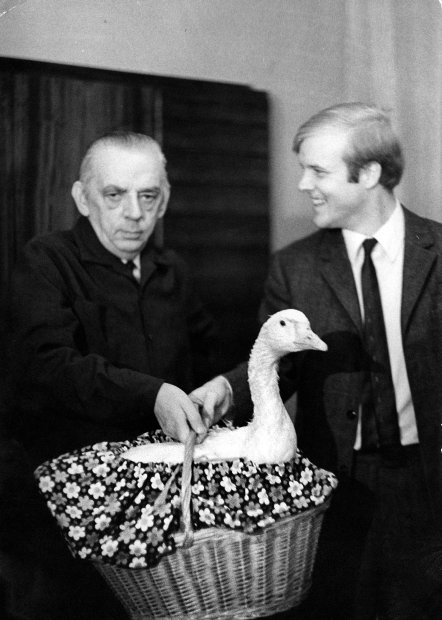
\includegraphics[width=.4\textwidth]{figures/mazur_goose_enflo.jpg}};
	\end{tikzpicture}
	\caption{Nel 1936 Mazur mise in palio un'oca `viva, e grassa' per la risoluzione del problema dell'approssimazione. Nel 1972, Enflo riceve dunque il suo premio.}
\end{figure}

\section{Elementi di teoria spettrale}
\begin{definition}
	Sia $E$ uno spazio di Banach, sia $T:E \to E$ lineare e continuo. Si chiama \defining{insieme risolvente} di $T$ l'insieme
	\begin{equation*}
		\rho(T) = \{\lambda \in \C \suchthat \text{$T-\lambda I$ è biettiva} \}.
	\end{equation*}
	In altre parole,
	\begin{equation*}
		\lambda \in \rho(T) \sse \text{per ogni $y \in E$ esiste $x \in E$ tale che $Tx - \lambda x = y$}.
	\end{equation*}
	Per $\lambda \in \rho(T)$, si dice \defining{operatore risolvente} associato l'operatore $(T-\lambda I)^{-1}$. Infine, si dice \defining{spettro} di $T$ l'insieme
	\begin{equation*}
		\sigma(T) = \C \setminus \rho(T).
	\end{equation*}
	Lo spettro puntuale di $T$ è l'insieme di tutti i suoi autovalori e si indica con $\sigma_p(T)$.
\end{definition}

\begin{remark}
	In dimensione finita, $\sigma = \sigma_p$, mentre in generale $\sigma_p \subseteq \sigma$.
\end{remark}

\begin{theorem}
\label{th:ops_five}
	Sia $E$ spazio di Banach, $T:E \to E$ lineare e continuo.
	Allora $\sigma(T)$ è chiuso e limitato, in particolare $\sigma(T) \subseteq B(0,\|T\|)$.
	Inoltre, se $E$ è complesso allora $\sigma(T) \neq \varnothing$.
\end{theorem}
\begin{proof}
	Per mostrare la chiusura di $\sigma(T)$, proviamo l'apertura di $\rho(T)$.
	Prendiamo allora $\lambda_0 \in \rho(T)$, $\lambda \in \C$ ed $y \in E$. Consideriamo l'equazione
	\begin{equation*}
		(T-\lambda I)(x) = y,
	\end{equation*}
	da cui
	\begin{eqalign*}
		Tx - \lambda x = y\\
		Tx - \lambda_0 x + \lambda_0 x - \lambda x = y\\
		(T-\lambda_0 I)x = y + (\lambda - \lambda_0) x\\
		x = (T-\lambda_0 I)^{-1}(y + (\lambda - \lambda_0)x)\\
		x = (\lambda - \lambda_0)(T-\lambda_0 I)^{-1}x + (T-\lambda_0 I)^{-1} y
	\end{eqalign*}
	che è un'equazione di punto fisso. Per il teorema del punto fisso di Banach--Caccioppoli\footnotemark, affinchè tale punto fisso esista  è sufficiente che l'operatore $(\lambda - \lambda_0)(T-\lambda_0I)^{-1}$ abbia norma strettamente inferiore di $1$, cioè che
	\begin{equation*}
		\lambda - \lambda_0 < \frac1{\|T-\lambda_0I\|}.
	\end{equation*}
	Dunque tutti i $\lambda$ in $B(\lambda_0, 1/\|T-\lambda_0I\|)$ sono risolventi, e quindi $\rho(T)$ è aperto.

	\footnotetext{\begin{theorem*}[Banach--Caccioppoli]
		Ogni contrazione (mappa lipschitziana con costante di Lipschitz $< 1$) di uno spazio metrico completo ammette un punto fisso, che si ottiene come limite della successione delle iterate di un punto qualunque.
	\end{theorem*}
	Il teorema ci permette di concludere che l'Italia in Miniatura ha un punto che è rappresentato da sè stesso. Per trovarlo, basta chiedere al bigliettaio dove sia la biglietteria, e così via.}

	Dimostriamo ora che $\sigma(T) \subseteq B(0, \|T\|)$.
	Sia $\lambda \neq 0$, $y \in E$, si ha
	\begin{eqalign*}
		Tx-\lambda x = y\\
		Tx = \lambda x + y\\
		\frac{Tx}\lambda = x+ \frac{y}\lambda\\
		\frac{Tx}\lambda - \frac{y}\lambda = x
	\end{eqalign*}
	che è ancora un'equazione di punto fisso. Ragionando come sopra, otteniamo che $\lambda \in \rho(T)$ se $\|T/\lambda\| < 1$, cioè se $\lambda > \|T\|$. Ma allora $\sigma(T) \subseteq B(0,\|T\|)$.

	Infine, si può dimostrare che l'operatore che associa $\lambda \in \rho(T)$ al suo operatore risolvente è analitica, e si può dimostrare che $\lim_{|\lambda| \to \infty} (T-\lambda I)^{-1} = 0$ poichè sappiamo che $\rho(T)$ è contenuta nel complementare di una palla. Da ciò segue che $\|T-\lambda I^{-1}\|$ è limitata.
	Ma se $\sigma(T) = \varnothing$, allora $\rho(T) = \C$ e siccome $\lambda \mapsto \|(T-\lambda I)^{-1}\|$ è analitica, dal teorema di Liouville otterremo che è costante. Siccome il limite è nullo, dovrebbe essere costantemente nulla, cioè $T-\lambda I = 0$, assurdo per un operatore invertibile.
\end{proof}

L'ultimo punto è falso in $\R$:

\begin{remark}
	Sia $T:\R^2 \to \R^2$ definito da
	\begin{equation*}
		Tx  = \begin{pmatrix}
			0 & 1\\
			-1 & 0
		\end{pmatrix}x
	\end{equation*}
	Allora $\sigma(T) = \pm i$ mentre è vuoto in $\R$.
\end{remark}

\begin{exercise}
	Sia $T: \ell^2 \to \ell^2$ l'operatore di backshift:
	\begin{equation*}
		T(x_1, x_2, x_3, \ldots) = T(x_2, x_3, \ldots).
	\end{equation*}
	Determinare $\sigma(T)$, $\sigma_p(T)$.

	\textbf{Svolgimento}.
	Si osservi innanzitutto che $\|T\| \leq 1$, d'altro canto $Te_2 = e_1$ dunque $\|T\| = 1$. Segue che $\sigma(T) \subseteq B(0,1)$. Lo spettro puntuale è invece dato da quelle quei $\lambda \in \C$ per cui
	\begin{equation*}
		(x_2, x_3, \ldots) = \lambda (x_1, x_2, \ldots).
	\end{equation*}
	cioè quando
	\begin{equation*}
		x_2 = \lambda x_1, \quad x_3 = \lambda x_2, \ldots
	\end{equation*}
	Allora scelto $x_1 \in \C$, le soluzioni hanno forma
	\begin{equation*}
		x_1 (1, \lambda, \lambda^2, \ldots)
	\end{equation*}
	che per essere in $\ell^2$ debbono avere $|x_1|^2\sum_{n=0}^\infty |\lambda|^{2n} < \infty$, da cui $|\lambda| < 1$. Per cui $\sigma_p(T) = B(0,1)$, ma $\closure{\sigma_p(T)} \subseteq \sigma(T)$, dunque $\sigma(T) = \closure B(0,1)$, ossia
	\begin{equation*}
		\sigma(T) \setminus \sigma_p(T) = \partial B(0,1).
	\end{equation*}
\end{exercise}

\begin{remark}
	Sia $E$ spazio di Banach, e supponiamo che $\dim E = \infty$. Sia inoltre $T:E \to E$ compatto. Allora $0 \in \sigma(T)$ siccome $T$ non è invertibile.
\end{remark}

\begin{theorem}[di Riesz--Schauder]
\label{th:riesz_schauder}
	Sia $E$ spazio di Banach e sia $T:E \to E$ compatto.
	Se $\dim E \lneq \infty$ allora $\sigma(T) = \sigma_p(T)$, mentre se $\dim E = \infty$ allora
	\begin{equation*}
		\sigma(T) = \{0\} \cup \underbrace{\{\lambda_1, \ldots, \lambda_n, \ldots\}}_{\text{autovalori al più numerabile}},
	\end{equation*}
	cioè $T$ ha \defining{spettro discreto} e gli autovalori non nulli hanno molteplicità finite, ossia $\dim \ker(T-\lambda I) \lneq \infty$.
	Inoltre, nel caso $\sigma(T)$ sia infinito, $\lambda_n \conv 0$.
\end{theorem}
\begin{proof}
	Omissis.
\end{proof}

\begin{lemma}
\label{lemma:ops_spectral_selfadjoint}
	Sia $H$ spazio di Hilbert, $T:H \to H$ autoauggiunto.
	Allora
	\begin{enumerate}
		\item gli autovalori di $T$ sono reali,
		\item autovettori relativi ad autovalori distinti sono ortogonali,
		\item e, nel caso $T$ sia compatto e $H\neq \{0\}$, uno tra $\|T\|$ e $-\|T\|$ è un autovalore di $T$.
	\end{enumerate}
\end{lemma}
\begin{proof}
	\leavevmode
	\begin{enumerate}
		\item Sappiamo che per $T$ autoauggiunto, $(Tx,x) \in \R$. D'altra parte da $Tx=\lambda x$ otteniamo che $(Tx,x) = \lambda (x,x)$ è reale, perciò necessariamente $\lambda \in \R$.
		\item Supponiamo che $x$ sia autovettore per $\lambda_1$ e $y$ per $\lambda_2 \neq \lambda_1$. Vale
		\begin{equation*}
			(\lambda_1 x, y) = (Tx, y) = (x, Ty) = (x, \lambda_2 y)
		\end{equation*}
		da cui $(\lambda_1 - \lambda_2)(x,y) = 0$ che implica $(x,y) = 0$ in quanto abbiamo supposto $\lambda_1 \neq \lambda_2$.
		\item Si può dimostrare che se $T$ è autoauggiunto, allora $\|T\| = \sup_{\|x\|=1} |(Tx,x)|$. Nel caso $T$ sia compatto e non banale, allora esiste una successione $\{x_n\}_{n \in \N}$ in $H$, di norma unitaria, tale che $|(Tx_n,x_n)| \conv \|T\|$.
		Salvo passare ad una sottosuccessione, $(Tx_n, x_n) \conv \|T\|$ o $-\|T\|$, Chiamiamo questo limite $\mu$. Si ha
		\begin{equation*}
			\|Tx_n - \mu x_n\|^2  = \|Tx_n\|^2 - 2 \mu \Re{Tx_n, x_n} + \mu^2 \|x_n\|^2 \leq \|T\|^2 - 2\mu \underbrace{(Tx_n, x_n)}_{\conv \mu} + \mu^2 \conv 0.
		\end{equation*}
		Per compattezza di $T$, a meno di passare ad una sottosuccessione, $Tx_n$ converge. Allora la convergenza di $Tx_n$ implica la convergenza di $\mu x_n$ (carabinieri). Segue che $x_n \conv x$, per cui $Tx_n - \mu x_n \conv Tx - \mu x = 0$, e $\|x\| =1$ dunque $x \neq 0$.
	\end{enumerate}
\end{proof}

Il seguente è un teorema spettrale per gli operatori compatti. Ne esiste una versione analoga per operatori non compatti, dimostrata da Stone, ed infine per operatori non limitati, dimostrato da Von Neumann.

\begin{theorem}[Il famoso teorema di Hilbert--Schmidt]
	Sia $T:H \to H$ un operatore compatto ed autoauggiunto su uno spazio di Hilbert $H$.
	Allora esiste una successione $\{u_n\}_{n \in \N}$ in $H$ di autovettori associati agli autovalori non nulli di $T$, tale che
	\begin{enumerate}
		\item $\{u_n\}_{n \in \N}$ è una base hilbertiana per $\closure{\im T}$.
		\item Se $\{\lambda_n\}_{n \in \N}$ è la successione degli autovalori associati agli $\{u_n\}_{n \in \N}$, ognuno ripetuto tante volte quanto è la sua molteplicità, allora
		\begin{equation}
		\label{eq:hilbert_schmidt}
			Tx = \sum_{n=1}^\infty \lambda_n\, (x,u_n)\,u_n.
		\end{equation}
	\end{enumerate}
\end{theorem}
\begin{remark}
	La~\eqref{eq:hilbert_schmidt} esprime il fatto che $T$ è diagonale rispetto alla base $\{u_n\}_{n \in \N}$!
\end{remark}
\begin{proof}
	Ricordiamo che $\closure{\im T} = (\ker T)^\perp$, e $H= \ker T \oplus \closure{\im T}$. Sia
	\begin{equation*}
		\Lambda = \{ \text{autovalori non nulli di $T$} \}
	\end{equation*}
	Abbiamo visto che $\dim \ker (T -\lambda I) = n_\lambda \lneq \infty$, per ogni autovalore $\lambda in \Lambda$. Dunque possiamo mettere insieme un insieme ortonormale numerabile andando a pescare una base ortonormale (finita) per ogni autospazio.
	Sia $U=\{u_n\}_{n \in \N}$ tale insieme, vogliamo provare che $\closure{\langle U \rangle} = \closure{\im T}$.
	È banale che $U \subset \im T$ ($Tx = \lambda x \implies x = T(x/\lambda) \in \im T$).
	Invece, supponiamo per assurdo che $\closure{\langle U \rangle } \subsetneq \closure{\im T}$. Siccome $\closure{\im T}$ è uno spazio di Hilbert, possiamo decomporlo come $\closure{\langle U \rangle} \oplus \closure{\langle U \rangle}^\perp$.
	Osserviamo che $T$ fissa $U^\perp$. Se $x \in U^\perp$ infatti, allora per ogni $y \in U$
	\begin{equation}
		(Tx,y) = (x,Ty) = (x, \lambda y) = \underbrace{\lambda}_{\in \R} \underbrace{(x,y)}_{x \perp y} = 0.
	\end{equation}
	Siccome $T$ è compatto ed autoauggiunto, e abbiamo supposto che $\langle U \rangle^\perp$ sia diverso da $\{0\}$, allora dal Lemma~\ref{lemma:ops_spectral_selfadjoint} otteniamo che esiste $u \in \closure{\langle U \rangle}^\perp$ autovettore non nullo di $T$ associato a $\pm \|T\vert_{\closure{\langle U \rangle}^\perp}\|$. Ciò contraddice la massimalità di $U$, e dunque $\closure{\langle U \rangle} = \closure{\im T}$, e quest'ultimo spazio è hilbertiano.

	Sia $x \in H$, siccome $Tx \in \im T$, dal punto precedente (e per il teorema di Fourier) sappiamo che
	\begin{equation*}
		Tx = \sum_{n=1}^\infty (Tx, u_n)\,u_n.
	\end{equation*}
	Infine,
	\begin{equation*}
		(Tx, u_n) = (x, Tu_n) = (x, \lambda_n u_n) = \lambda_n (x, u_n)
	\end{equation*}
	e ciò conclude la dimostrazione.
\end{proof}

\begin{corollary}
	Se $T:H \to H$ è compatto ed autoauggiunto, allora $H$ possiede una base hilbertiana di autovettori di $T$.
\end{corollary}
\begin{proof}
	Infatti $H = \ker T \oplus \closure{\im T}$. Per il teorema precedente, $\closure{\im T}$ ha una base hilbertiana numerabile di autovettore, mentre $\ker T$ ha una base hilbertiana in quanto sottospazio chiuso in uno spazio di Hilbert. Siccome $\ker T$ è un autospazio per $T$, la tesi è provata.
\end{proof}

\begin{remark}
	Si noti che la decomposizione $H = \ker T \oplus \closure{\im T}$ associata ad un operatore compatto ed autoauggiunto esibisce $H$ diviso in una parte separabile (l'immagine, che ha una base hilbertiana numerabile) ed una non separabile. Chiaramente $\closure{\im T}$ non è necessariamente massimale.
\end{remark}

\begin{theorem}[dell'alternativa di Fredholm]
	Sia $T:H \to H$ compatto e autoauggiunto. Consideriamo le seguenti equazioni:
	\begin{equation*}
		(1)\ x - Tx = 0, \qquad (2)\ x-Tx = y.
	\end{equation*}
	Allora vale una e una sola delle seguenti alternative:
	\begin{enumerate}
		\item La $(1)$ ha solo la soluzione nulla, nel qual caso $(2)$ ha una e una sola soluzione per ogni $y \in H$.
		\item La $(1)$ ha soluzione non nulla, nel qual caso $(2)$ ha soluzione se e solo se $y$ è ortogonale a tutte le soluzioni di $(1)$.
		Inoltre se vi è una soluzione allora ce ne sono infinite.
		Infine, lo spazio di tali soluzioni è chiuso.
	\end{enumerate}
\end{theorem}
\begin{proof}
	Si assuma che $(1)$ abbia solo la soluzione nulla. Ciò significa che $1 \notin \sigma_p(T)$, e dunque $1 \notin \sigma(T)$, e quindi $I-T$ è invertibile e la $(2)$ ha sempre una soluzione unica.

	Supponiamo invece che $(1)$ abbia soluzione non nulle, da cui $1 \in \sigma_p(T)$ e $\ker (I-T) \neq \{0\}$. Allora $H = \ker (I-T) \oplus \closure{\im (I-T)}$. Allora se $y \in \im(I-T)$, $y \perp \ker (I-T)$, cioè che se la $(2)$ ha soluzione per $y$ allora $y$ è ortogonale alle soluzioni di $(1)$.
	Proviamo ora che se $y \in (\ker(I-T))^\perp$, allora $y \in \im(I-T)$. Da questo discende anche che $\im(I-T)$ è chiuso, in quanto complemento ortogonale.
	Usiamo Hilbert--Schmidt per ottenere una base hilbertiana di autovalori di $T$ per $\closure{\im T}$. Per cui nella $(2)$ poniamo
	\begin{equation*}
		x = x_0 + x_1, \quad y=y_0+y_1
	\end{equation*}
	dove $x_0,y_0 \in \ker T$ e $x_1,y_1 \in \closure{\im T}$. Del resto
	\begin{equation*}
		x = x_0 + \sum_{n=1}^\infty (x, u_n)\,u_n, \qquad y = y_0 + \sum_{n=1}^\infty (y, u_n)\,u_n
	\end{equation*}
	e l'equazione diventa
	\begin{equation*}
		x_0 + \sum_{n=1}^\infty (x, u_n)\,u_n - \sum_{n=1}^\infty \lambda_n (x,u_n) u_n = y_0 + \sum_{n=1}^\infty (y, u_n)\,u_n
	\end{equation*}
	cioè
	\begin{equation*}
		(2) \iff
		\begin{cases}
			x_0 = y_0,\\
			(1-\lambda_n)(x,u_n) = (y,u_n)
		\end{cases}
	\end{equation*}
	Quindi se $\lambda_n =1$, $(y,u_n) = 0$. Ma infatti $y \in \ker(I-T)$, che è l'autospazio relativo a $1$.
	Se invece $\lambda_n \neq 1$, si ottiene
	\begin{equation*}
		(x,u_n) = \frac{(y,u_n)}{1-\lambda_n}
	\end{equation*}
	che mi permette di ottenere $x$, siccome la successione $(y,u_n)/(1-\lambda_n)$ è in $\ell^2$ (perchè $\lambda_n \conv 0$, quindi $1-\lambda_n$ è in $\ell^\infty$, ed $(y,u_n) \in \ell^2$).
\end{proof}
